% twocolumn を使うと2段組になる

%\documentclass[a4j,twocolumn]{jsarticle}        % -> platex
%\documentclass[a4j,twocolumn]{ujarticle}       % -> uplatex
\documentclass[uplatex]{jsarticle}   % -> uplatex + jsarticle

\usepackage{resume} % 他パッケージ,専用コマンド,余白の設定が書かれている

%%%%%%%%%%%%%%%%%%%%%%%%%%%%%%%%%%%%%%%%%%%%%%%%%%%%%%%%%%%%%%%%%%%%%%%%
% ヘッダ: イベント名,日付,所属,タイトル,氏名
%%%%%%%%%%%%%%%%%%%%%%%%%%%%%%%%%%%%%%%%%%%%%%%%%%%%%%%%%%%%%%%%%%%%%%%%


\pagestyle{plain}

\begin{document}
\twocolumn[
    \beginheader{令和4年度 コンピュータサイエンス学部 輪講発表}{2022}{12}{15}{井上 研究室}
    \title{モーションベースを用いた仮想空間における歩行体験の評価}
    \author{C0B20046 川東隆継 (Takastugu Kawahigashi)}
    \endheader
]
\vspace{3mm}

%%ページ番号
\setcounter{page}{1}

\section{はじめに}

現実世界において歩行は人間の活動に欠かせない移動手段の一つであり,VRでもコンテンツの種類を問わず多く登場する.従来ではロコモーションインターフェイスのGaitMaster\cite{文献2}のフットパッド型や,ATLAS\cite{文献3}のトレッドミル型などの大掛かりな装置を用いることが多い.

近年では身体的負荷の低さや姿勢の汎用性にメリットがある座位姿勢で利用するものも提案されているが立位姿勢と比較して歩行感覚が生まれにくいという指摘もある.


特に本研究で着目したモーション
ベースは,前庭感覚を人工的に提示する前庭感覚ディ
スプレイの一種であり,人間の体全体を動かすこと
で前庭感覚を提示する装置である.座位姿勢で利
用するシート型のものが既に広く利用されており,乗り
物表現に強いのが特徴だが,前述のように歩行時の振
動を再現した例など,多様な使途が検討されている.


そこで本研究では,座位姿勢での仮想歩行体験について,そのユーザ体験を総合的に評価した.特にVRコンテンツへの適用を目的とし,モーションベースによる歩行振動,足ふみ操作,及び仮想の歩行者の存在がユーザー体験に与える影響を検証した.


\section{実験装置・環境}
\figref{fig:my_label},\figref{fig:my_label_2}に本実験の実験環境と仮想空間の様子を示す.
本実験ではエアコンプレッサ式のモーションベースを使用し,VR視聴用のHMDにはアイトラッキング機能を有するVive Pro Eyeを用いた.

本実験はモーションベースが稼働するのに十分なスペースを確保できる環境で行い,実験者はモーションベースの可動域外にて実験刺激を操作した.


\begin{figure}[t]
    \centering
    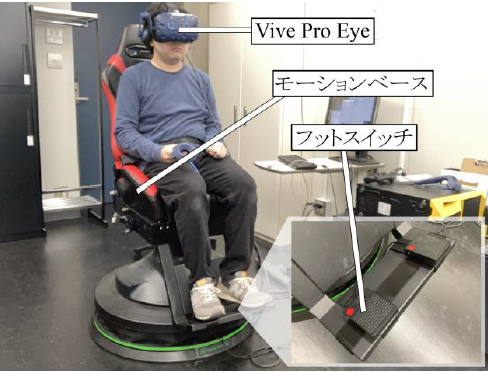
\includegraphics{reinkou_figure_1.png}
    \caption{実験環境}
    \label{fig:my_label}
\end{figure}

\begin{figure}[t]
    \centering
    \includegraphics{rinkou_figure_5.png}
    \caption{本実験の仮想空間}
    \label{fig:my_label_2}
\end{figure}



\section{実験}
\subsection{概要}
実験条件は以下の\tabref{tab:fonts}に示すように歩行時振動,足踏み操作,
仮想の歩行者の有無の組み合わせが異なる条件1から条件4までの4条件であった.
なお,順序効果の影響を排除するため,体験する条件の順番は参加者によりランダマイズされた.


評価方法はアンケート,インタビューによって行った.
\begin{table}
  \centering
  % \scriptsize
  \caption{実験条件}
  \label{tab:fonts}
  \begin{tabular}[t]{|l|l|l|l|l|}
    \hline
     & 条件 & 条件 & 条件 & 条件\\
     & C1 & C2 & C3 &C4\\
    \hline
    歩行時振動 &なし&あり&あり&あり\\
    \hline
    足ふみ操作&なし&なし&あり&あり\\ 
    \hline
    仮想の歩行者&いない&いない&いない &いる\\
    \hline
  \end{tabular}
\end{table}


\subsection{足踏み操作の有無}
足踏み操作がある条件では,参加者が左右のフットスイッチを交互に踏むことで仮想空間内を前進し,両方を踏むことで停止した.歩行時振動や足音の間隔は参加者の足踏みに同期させた.

足踏み操作がない条件では,自動的に仮想空間内
を前進した.参加者は両方のフットスイッチを踏んだまま
で刺激を体験した.

\subsection{仮想の歩行者の有無}
仮想の歩行者がいる条件では,仮想空間内に仮想
の歩行者を7体配置した.うち5体は参加者の前方か
ら参加者とすれ違い,2体は後方から参加者を追い抜
くようにした.



\subsection{実験手順}
\figref{fig:my_label_4}に実験手順を示す。実験前にはキャリブレーシ
ョンとして,Vive Pro Eyeのアイトラッキング機能のキャリ
ブレーションと,参加者の平均的な足踏み時間の測定
を実施したのち,足踏み操作の練習を十分に行った.
本試行は4回行われた.各試行後にはHMDを装着し
たままアンケートとインタビューへの回答を行ったうえで,参加者がVR酔いの症状や疲労感を自覚していれば適宜休憩を挟み,次の試行へと移った.

\begin{figure}[h]
    \centering
    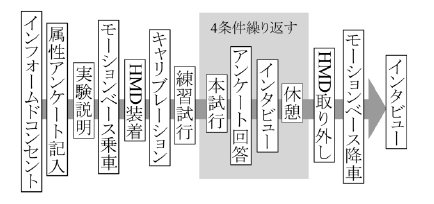
\includegraphics{rinkou_figure_4.png}
    \caption{実験環境}
    \label{fig:my_label_4}
\end{figure}
\section{実験結果}

\subsection{アンケート}
VR酔いに関する質問では,条件C2のスコアが他の条件と比較して有意に高かった.SAM\cite{文献18}情動価の結果では,条件C2のスコアが,条件C3,C4と比較して有意に低かった.SAM覚醒度の結果では,歩行時振動のある条件で有意に高かった.
歩行感覚に関する質問では すべての質問について,足踏み操作のある条件で有意に高かった.
仮想空間の認識に関する質問のうち,距離感覚と自身のスケール感では,条件間の有意差は確認できなかった.
速度感覚に関する質問では,条件C2のスコアが条件C3のスコアと比
較して有意に高い傾向があった.条件C1,C4では実際歩行に近い速度知覚が得られていた.


\section{おわりに}
本研究では座位姿勢での仮想空間における歩行体
験について歩行時振動,足踏み操作,仮想空間内に配置された仮想の歩行
者という条件の組み合わせでユーザーにおける影響を図った.

その結果歩行時振動,足踏み操作,仮想空間内に配置された仮想の歩行
者がユーザ体験に多様な変化,影響を与えることが明
らかになった.
したがって,コンテンツ制作にあたっては
その制作意図に合わせて,装置や映像の構成要素を
取捨選択することが重要であると考えられた.

第1章で述べた通り,仮想空間内で歩行するインタ
ーフェイスや歩行感覚を提示する装置は古くから研究
が進められてきており,これまで様々な種類が提案され
ている.しかし,それらの適切な利用方法や組み合わせ
方などの,コンテンツレベルでの方法論については研
究が進んでおらず,確立されていないのが現状である.
したがって,より実用に近いコンテンツレベルの研究が
将来のVRコンテンツの発展には必要である.実際に本
研究からも多くの検討課題が得られ,今後も研究を進め
ていく必要があると考える.







%---------------------------------------------------------------------------
% 本文終わり
%---------------------------------------------------------------------------

 % 参考文献
\bibliographystyle{junsrt}
\bibliography{ref}


\end{document}


%-----------------------------------------------------
% テンプレート
%------------------------------------------------------------------------------

%-----------
%% 箇条書き
%-----------
%\begin{itemize}
% \item
%\end{itemize}

%-------------------
%% 番号付き箇条書き
%-------------------
%\begin{enumerate}
% \item
%\end{enumerate}

%-----------
%% 図の表示
%-----------
%\begin{figure}[H]
% \centering
% \includegraphics[clip,width=7cm]{hoge.eps}
% \caption{図タイトル}\label{fig:hoge}
%\end{figure}

%-----------
%% 図の参照
%-----------
%\figref{fig:hoge}

%-----------
%% 表の作成
%-----------
%\begin{table}[H]
% \centering
% \caption{表タイトル}\label{tab:fuga}
% \begin{tabular}{|c|c|c|}\hline
%  hemo & piyo & fuga \\ \hline
%  hemo & piyo & fuga \\ \hline
% \end{tabular}
%\end{table}

%-----------
%% 表の参照
%-----------
%\tabref{tab:fuga}

%-----------
%% 参考文献
%-----------
%\begin{thebibliography}{9}
% \bibitem{piyo} 参考文献
%\end{thebibliography}

%-----------------
%% 参考文献の参照
%-----------------
%\cite{piyo}
